%%%%%%%%%%%%%%%%%%%%%%%%%%%%%%%%%%%%%%%%%%%%%%%%%%%%%%%%%%%%%%%%%%%%%%%%%
%%%%%%%%%%%%%%%%%%%%%%%%%%%%%%%%%%%%%%%%%%%%%%%%%%%%%%%%%%%%%%%%%%%%%%%%%
%%%%%%%%%%%%%%%%%%%%%%%%%%%%%%%%%%%%%%%%%%%%%%%%%%%%%%%%%%%%%%%%%%%%%%%%%

\begin{frame}{What makes an estimator non-robust?  A tail sum.}

Report non-robustness if
$ \Delta \le \thetafunlin(\w^*) - \thetafun(\onevec)  =
\color{red}- \sum_{n=1}^{\lfloor \alpha N \rfloor} \infl_{(n)}$.

\pause
Robustness is determined by a tail sum of the influence scores.

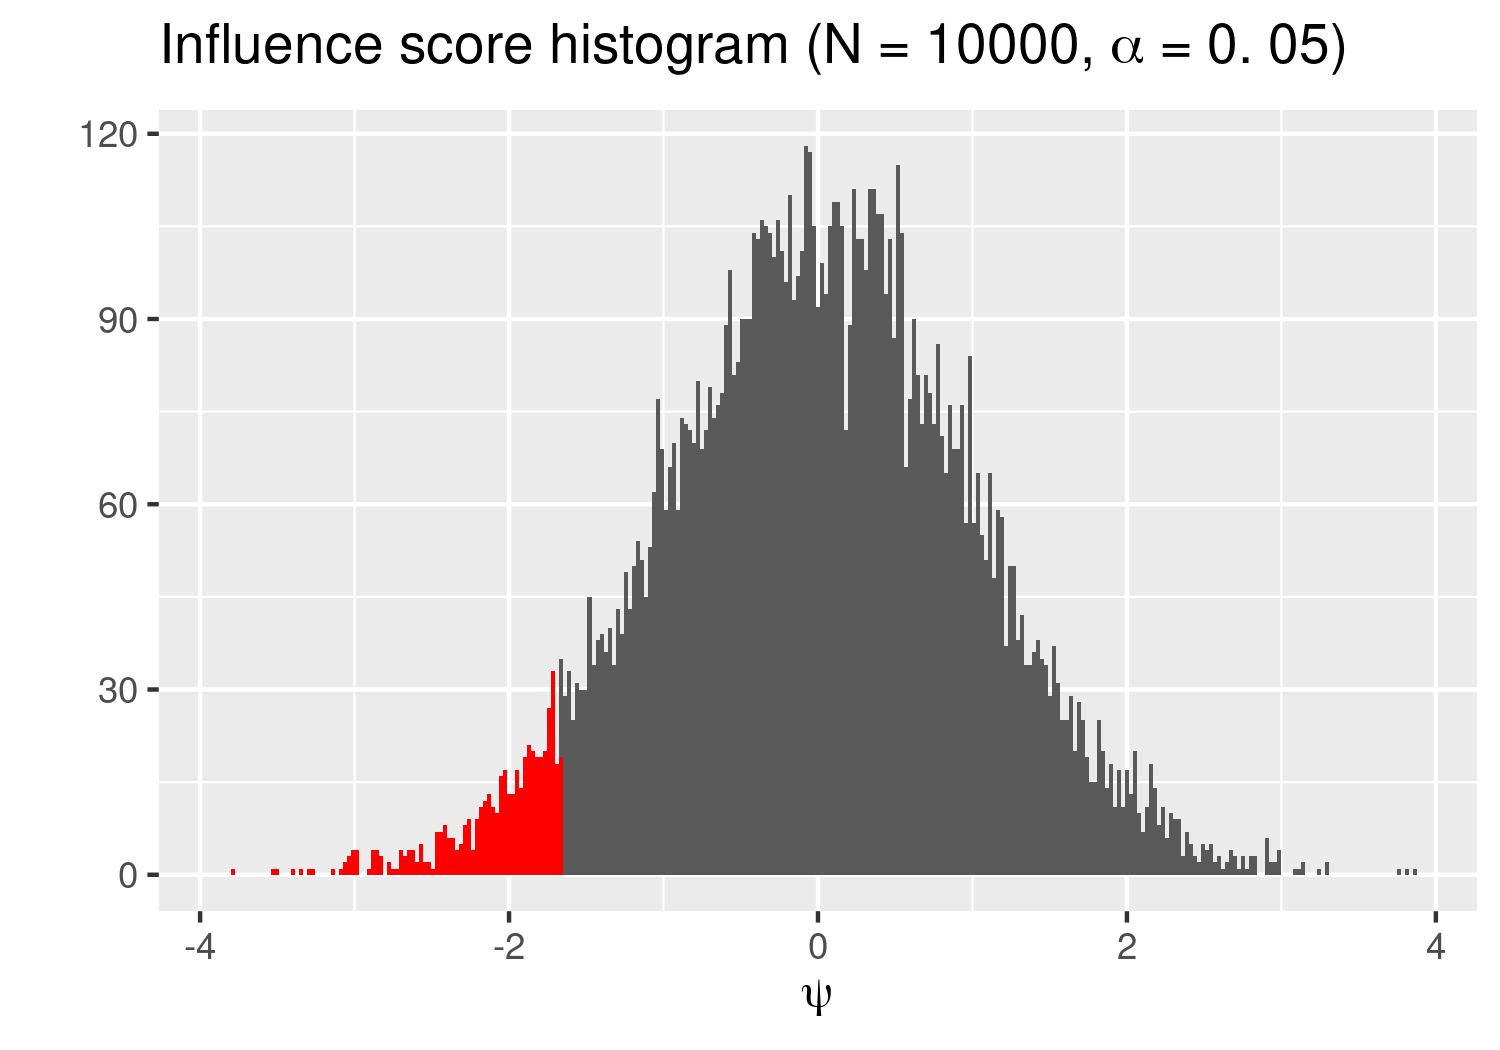
\includegraphics[width=0.9\linewidth]{static_figures/simple_infl_example.png}


\end{frame}

%%%%%%%%%%%%%%%%%%%%%%%%%%%%%%%%%%%%%%%%%%%%%%%%%%%%%%%%%%%%%%%%%%%%%%%%%
%%%%%%%%%%%%%%%%%%%%%%%%%%%%%%%%%%%%%%%%%%%%%%%%%%%%%%%%%%%%%%%%%%%%%%%%%
%%%%%%%%%%%%%%%%%%%%%%%%%%%%%%%%%%%%%%%%%%%%%%%%%%%%%%%%%%%%%%%%%%%%%%%%%

\begin{frame}{A decomposition of the tail sum of influence scores.}

Report non-robustness if
\begin{align*}
    \vspace{-1em}
\Delta \le{}& - \sum_{n=1}^{\lfloor \alpha N \rfloor} \infl_{(n)}
\onslide<3->{
= \hat\sigma_\phi
    \left(
        - \frac{1}{N} \sum_{n=1}^{\lfloor \alpha N \rfloor}
        \frac{N \infl_{(n)}}{\hat\sigma_\phi}
    \right)
}
\onslide<5->{
 = \hat\sigma_\phi \hat\Gamma_\alpha
}
% \onslide<6->{
% \quad \Leftrightarrow \quad \\
% \color{red}
% \frac{\Delta}{\hat\sigma_\phi} \le{}& \Gamma_\alpha
% \quad\textrm{where } \frac{\Delta}{\hat\sigma_\phi} =
%     \textrm{ ``Signal to noise ratio''}
% }
\end{align*}
%\vspace{-1em}

% $ \Delta \le - \sum_{n=1}^{\lfloor \alpha N \rfloor} \infl_{(n)}$
% \onslide<3->{
% $= \hat\sigma_\phi
%     \left(
%         - \frac{1}{N} \sum_{n=1}^{\lfloor \alpha N \rfloor}
%         \frac{N \infl_{(n)}}{\hat\sigma_\phi}
%     \right)$
% }
% \onslide<5->{
% $ = \hat\sigma_\phi \hat\Gamma_\alpha$
% }
% \onslide<6->{
% $\quad \Leftrightarrow \quad$\\
% $\color{red}
% \frac{\Delta}{\hat\sigma_\phi}
% \le \Gamma_\alpha$
% }

%\vspace{1em}
\begin{columns}
\begin{column}{0.45\linewidth}
\onslide<2->{
Fact 1: \citep{hampel1986robustbook}\\
$\underbrace{\frac{1}{N} \sumn (N \infl_n)^2}_{\hat\sigma_\phi^2 \textrm{: the ``noise''}}
    \rightarrow \mathrm{Var}\left( \sqrt{N} \thetafun \right)$
}
\end{column}

\begin{column}{0.45\linewidth}
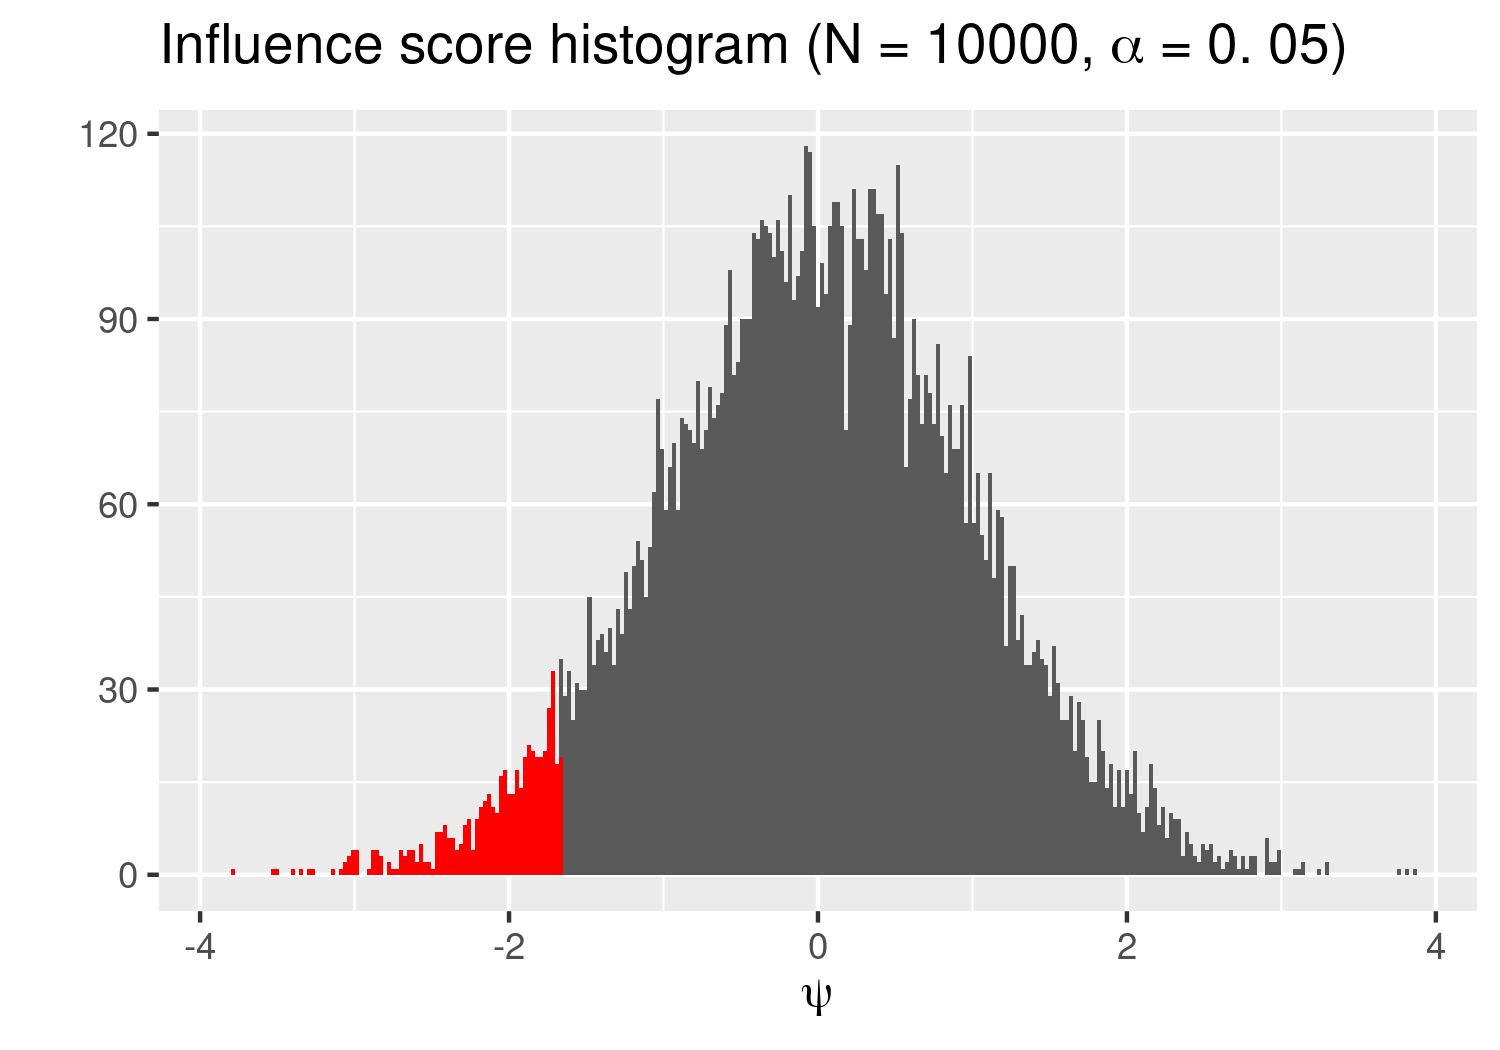
\includegraphics[width=0.8\linewidth]{static_figures/simple_infl_example.png}
\end{column}
\end{columns}

\begin{columns}
\begin{column}{0.45\linewidth}
\onslide<4->{
Fact 2: (Cauchy-Schwartz)
$\underbrace{
- \frac{1}{N}
    \sum_{n=1}^{\lfloor \alpha N \rfloor} \frac{N \psi_{(n)}}{\hat\sigma_\phi}
}_{\hat\Gamma_\alpha \textrm{: the ``shape''}}
\le \sqrt{\alpha}
$
}
\end{column}

\begin{column}{0.45\linewidth}
\onslide<5->{
%\vspace{-1em}
Fact 3:\\
Under standard conditions, \\
$\hat\sigma_\phi$ and $\hat\Gamma_\alpha$
converge to nozero constants.
}
\end{column}

\end{columns}

\end{frame}


%%%%%%%%%%%%%%%%%%%%%%%%%%%%%%%%%%%%%%%%%%%%%%%%%%%%%%%%%%%%%%%%%%%%%%%%%
%%%%%%%%%%%%%%%%%%%%%%%%%%%%%%%%%%%%%%%%%%%%%%%%%%%%%%%%%%%%%%%%%%%%%%%%%
%%%%%%%%%%%%%%%%%%%%%%%%%%%%%%%%%%%%%%%%%%%%%%%%%%%%%%%%%%%%%%%%%%%%%%%%%

\begin{frame}{Corollaries.}
% Recall:
\begin{itemize}
    \item[] $\Delta$  = The signal = The change in $\phi$ that would alter your conclusion
    \item[] $\hat\sigma_\phi$ = The noise = A consistent estimator of $\mathrm{Var}(\sqrt{N}\phi)$
    \item[] $\hat\Gamma_\alpha$ = The shape = Converges to a nonzero constant, $\le \sqrt{\alpha}$
\end{itemize}

Report non-robustness if the \textbf{``signal to noise ratio''}
$\frac{\Delta}{\hat\sigma_\phi} \le \hat\Gamma_\alpha$.

\pause
\vspace{0.5em}
\textbf{Corollary:  Non-robustness possible even with correct specification.}
\vspace{-0.4em}
The noise $\hat\sigma_\phi$ may be larger than the effect
$\Delta$ you're trying to measure.

\pause
\vspace{0.5em}
\textbf{Corollary:  Leave-$\lfloor \alpha N \rfloor$-out robustness does not vanish as $N \rightarrow \infty$.}
\vspace{-0.4em}

Both $\hat\Gamma_\alpha$ and $\hat\sigma_\phi$ typically converge to nonzero constants.

\pause
\vspace{0.5em}
\textbf{Corollary:  Leave-$\lfloor \alpha N \rfloor$-out is different from standard errors.}
\vspace{-0.4em}

Standard errors reject when
$\frac{\Delta}{\hat\sigma_\phi} \le \frac{1.96}{\sqrt{N}} \ne \hat\Gamma_\alpha$.

\pause
\vspace{0.5em}
\textbf{Corollary:  Insignificance is always non-robust.}
\vspace{-0.4em}

Take $\Delta = \frac{1.96 \hat \sigma_\phi}{\sqrt{N}}$.  We report
non-robustness when $\hat\Gamma_\alpha \ge \frac{1.96}{\sqrt{N}} \rightarrow 0$.

\end{frame}


%%%%%%%%%%%%%%%%%%%%%%%%%%%%%%%%%%%%%%%%%%%%%%%%%%%%%%%%%%%%%%%%%%%%%%%%
%%%%%%%%%%%%%%%%%%%%%%%%%%%%%%%%%%%%%%%%%%%%%%%%%%%%%%%%%%%%%%%%%%%%%%%%
%%%%%%%%%%%%%%%%%%%%%%%%%%%%%%%%%%%%%%%%%%%%%%%%%%%%%%%%%%%%%%%%%%%%%%%%


\begin{frame}{Dropping data: Mexico Microcredit}

\MicrocreditMexicoGraphics{}

% \begin{tabular}{ll}
% { \footnotesize \textbf{Blue line:}}  &       {\footnotesize Original estimate} \\
% { \footnotesize \textbf{Red line:}}  &        {\footnotesize Estimate after removing points} \\
% { \footnotesize \textbf{Shaded bands:}}  &    {\footnotesize Standard errors}
% \end{tabular}

\textbf{Leave-$\alpha$-out robustness does not vanish as $N \rightarrow \infty$.}\\
\textbf{Leave-$\alpha$-out is different from standard errors.}\\
\textbf{Insignificance is always non-robust.}

\end{frame}
